\chapter{Introduction}


%Structuur volgens Erwin
% INLEIDING (10-15 p)
% Onderzoeksgebied (1-2 p)
% Motivatie, probleemstelling (3p)
% Overkoepelende doelstelling en 4 meer toegespitste onderzoeksvragen (0.5 p)
% Kort literatuuroverzicht over de belangrijkste thema's die in meerdere hoofdstukken terugkomen (fragiliteit, geweld, behavioral economics, risico, ...) (3p)
% Belangrijkste resultaten per paper en "contributie aan literatuur" (1-2 p)
% Belangrijkste methoden en waarom juist deze? (2p)
% Roadmap to the thesis (1 p)



\section{Problem Statement and Research Area}
% Onderzoeksgebied (1-2 p)
% Motivatie, probleemstelling (3p)

%https://nsdsguidelines.paris21.org/node/291
%https://papers.ssrn.com/sol3/papers.cfm?abstract_id=2622220


%markets:
%https://link.springer.com/article/10.1007/s10551-010-0402-8
%https://www.oecd-ilibrary.org/content/paper/5k49dfg9fb6d-en
%https://www.worldbank.org/en/topic/fragilityconflictviolence/overview

%problem statement/Hook
Between 1990 and 2015, the share of Africans living in absolute poverty fell from 54\% to 41\% \citep{Beegle2019}. However, because of population increase in the continent, the absolute number of Africans living in poverty has also increased; meanwhile, given the reductions in poverty elsewhere in the world, the proportion of the world's poor who live in Africa has increased in that time period.  Moreover, the poverty rates within Africa haven't declined uniformly across countries, with some countries faring worse than others. This means that the global poor are increasingly concentrated in a limited number of countries. The World Bank expects that by 2030, up to two thirds of the world's extremely poor live in Fragile Conflict-affected settings \citep{WorldBank2019}. %This does not make this a localized issue: instability in one country may have effects throughout the region through increased numbers of refugees and proliferation of armed groups. Such flows may even destabilize countries further away. %Climate change is expected to increase this instability further \citep{Burke2009}.

%some risks and drivers here.
\todo{Write a section on risks and drivers to development. These should be addressed in the thesis.}
Agriculture; Human Rights.

In order to address poverty at a global scale, a thorough understanding of development at a local scale, particular to this limited set of countries, is thus required. The constituent chapters of this dissertation aim to contribute to our knowledge of the dynamics behind development in selected countries in Africa. I present micro-level evidence from Sierra Leone, Cameroon and the Democratic Republic of the Congo (DRC). %In each chapter, I examine a different aspect of development; the link between these chapters is outlined in the Theoretical Framework below.   

\todo{Write a short background of the research area.}
\subsection{Sierra Leone}
In 2010, the year when the Sierra Leonean data for this thesis was collected, the largest development challenge was recovering from the war \todo{some more on the war, based on things below}. Agriculture, the largest sector in the country was hard-hit, leading to a high depedence on imported foodstuffs \citep{FAO2005}. The human toll of the war was high \todo{Expand this}.


\subsection{DR Congo}
The second area of focus for this dissertation is the Eastern part of the DRC, in particular South Kivu. The area has long lagged behind in various metrics of human development. \todo{what metrics?} Improving this situation is complex. Firslty, even XX years after the offcial end of the Second Congo War there are still armed groups active in the region. \todo{which groups and how active are they} Secondly, the quality of governance in the area is low. \todo{examples; ethicity and elections} 


due to conflict and poor governance. The province was a major flashpoint in the first and second Congo War. The conflict has had a severe impact on the people of South Kivu; the conflict saw widespread loss of live (both due to violence and deprevation) and human rights abuses. The effects of this can be seen today. 

\subsection{Cameroon}
The third area of focus is the Adamawa region in Northern Cameroon. The Adamawa region is mostly rural, with low population densities. The predominant source of income is agriculture. The most pressing development challenge of the region is its remoteness. Most household in our study sample live in small villages, with nearby markets their most accessible connection to the world at large. \todo{expand this; must be an old version of the paper lying around with more info.}

\section{Research Question}
% Overkoepelende doelstelling en 4 meer toegespitste onderzoeksvragen (0.5 p)
\todo{Write this into a story}
The three research areas of this disseration present different experiences with development. Each area has different risks and opportunities, as well as different development outcomes that are seen as priorities. The effect of each of these risks and opportunities on development outcomes is not direct. The effect is mediated through factors at the local or even the individual level, which in Figure \ref{intro:fig:framework} I capture under the term Social Capital (for a more thorough review see below). The importance of these local and individual factors underlines the need for micro-level data collection to shed light on these dynamics. The chapters of this dissertation each discuss a different aspect of the interplay between risks, opportunities, social capital and development outcomes. The questions they answer are as follows.
\begin{enumerate}
	\item What is the relationship between conflict and competitive behaviour? (Chapter \ref{chap:slfootball});
	\item What is the effect of input subsidies on novel technology adoption? (Chapter \ref{chap:n2a_impact});
	\item What is the effect of market access on trusting behaviour (Chapter \ref{chap:cameroontrust}); and,
	\item What are the drivers of sexual and gender-based violence in Eastern Congo (Chapter \ref{chap:congogbv}).
\end{enumerate}


\section{Literature Review}
% Kort literatuuroverzicht over de belangrijkste thema's die in meerdere hoofdstukken terugkomen (fragiliteit, geweld, behavioral economics, risico, ...) (3p)
Figure \ref{intro:fig:framework} outlines the relationships between the main topics of this dissertation. On the right-hand side, there are two indicators for development that are present in the areas of interest in this disseration: human rights and (agricultural) productivity. On the left, there are three risks and opportunities: violent conflict, markets, and development aid. These risks and opportunities do not translate directly in development outcomes; rather, they are mediated through social capital and institutions.

\begin{figure}[htb]
  \centering
  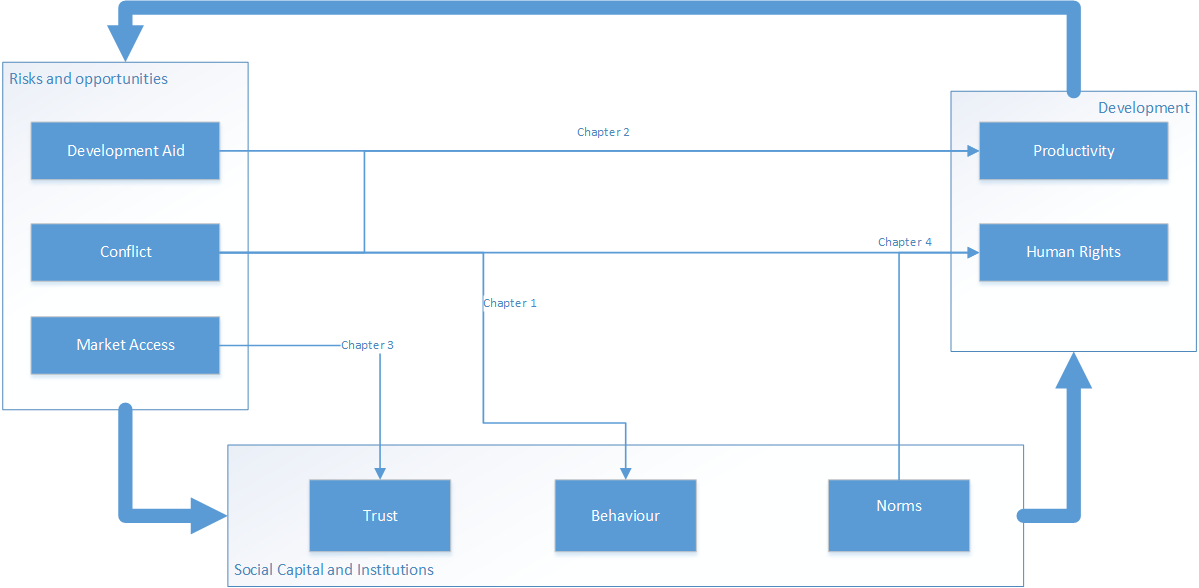
\includegraphics[width=0.8\linewidth]{"\git/thesis/analysis/introduction/figures/conceptual_framework.png"}
  \caption{Conceptual Framework}
  \label{intro:fig:framework}
\end{figure}

\subsection{Risks and Opportunities}\
As for the risks and opportunities to development I consider, the first is violent conflict. The risk posed by conflict to development were expressed by \citet{Collier2003}, by labelling conflict ``Development in Reverse''. The World Bank further underscored the importance of violent conflict poses in shaping development outcomes by titling their 2011 World Development Report ``Conflict, Security, and Development'' \citep{WorldBank2011}. Aside from the human rights violations that are inherent to violent conflict, other consequences include: decreased economic activity \citep{Collier1999} deforestation \cite[e.g.][]{Connectiona}, long-term incidence of domestic violence \citep[e.g.][]{LaMattina2017, Muller2019}, (mental) health problems \cite[e.g.][]{Smith2002, Iqbal2006a,Akresh2011} and food insecurity \cite[e.g.][]{Lecoutere2005, Verwimp2012}. However, some effects which may have some benefit to long-term development have been described, such as increased collective action \citep{Bellows2009b}, political participation \citep{Blattman2009a} and increased pro-social behaviour \citep{Voors2012a}.

Among the countries where data collection was done for this dissertation, two are post-conflict countries in Africa: Sierra Leone and DRC. The conflicts have had far-reaching effects. In Chapter \ref{chap:slfootball}, I examine some of the impacts that conflict has had on the behaviour of youths in Sierra Leone. Chapters \ref{chap:n2a_impact} and \ref{chap:congogbv} are set in DRC. The former focuses on agricultural productivity, which has suffered from the conflict; while the latter focuses on women's rights. %\todo{dit kan uitgebreider met meer focus op de theorie (dwz link met voorgaande paragraaf)}

Next, I consider an opportunity for development: markets. Markets provide opportunities for exchange and specialization, which can boost economic development. At the national level, trade is seen as a promising way to increase productivity in developing economies. Dutch development aid, for example, has a large focus on the complementarities between trade and development as a way of increasing investments and thus productivity \citep[see e.g.][]{Zoomers2014}. Aside from these impacts on the national level, increased access to markets have been shown to have effects at the local and individual level as well: markets are associated with trust \citep{Tu2010,Fischer2008}; increased rationality \citep{List2008,Cecchi2013,Braga2009} and decreases in risk aversion \citep{Melesse2015}. This corresponds with findings that from large-scale societies (which include markets) engage more in pro-social behaviour \cite{Henrich2005,Henrich2010}. These national and individual effects make that markets are an important consideration in analysing the development process. 

Chapter \ref{chap:cameroontrust} expands on this literature on the effects of markets on behaviour. Specifically, in the chapter I analyse how trust is shaped by the presence of local markets. The effect markets have mean they are more than a conduit for buying and selling goods, but can have deep impacts on societies.

%put in for development aid vs institutional reform: https://www.aeaweb.org/articles/pdf/doi/10.1257/jel.44.4.973
Thirdly, I consider development aid. At the turn of the century, the Millennium Development Goals were adopted in the hopes that the world's poorest countries (particularly in Africa) could be lifted out of poverty with a large-scale international effort. The underlying assumption was that a core challenge to African economies were adverse geographical conditions which hinder growth; ambitious investments by the international development community could then help increase agricultural productivity and decrease the impact of tropical diseases \citep{Sachs2005}. This push came out of disappointment with the levels of growth in the 1990s. The mantra of "stabilize, privatize and liberalize", as preached by the IMF and the World Bank, proved insufficient to achieve preferred development outcomes, leading to calls  for an increase in the levels of development aid \citep{Rodrik2006a}. However, increased calls for more direct intervention were not the only response to this disappointment: concurrently there was doubt about development aid's capability to achieve meaningful growth. \citet{Easterly2007} labels Development Assistance a ``mistake'', claiming that ``we don't know what actions achieve development''. A large literature has since sprung up that aims to fill exactly that knowledge gap and find out which development interventions work, and which don't. Improvements in statistical techniques and data collection methods have allowed development economists to get more accurate assessments of the impact of aid programs. Academics and development NGOs have embraced methods such as Randomized Controlled Trials (RCTs) to find out what works and what doesn't \citep[see e.g.][]{Bannerjee2011}.  

This dissertation follows in this tradition. Chapter \ref{chap:n2a_impact} is about the impact evaluation of an agricultural intervention, and both Chapters \ref{chap:cameroontrust} and \ref{chap:congogbv} were funded by being smaller parts of similar impact evaluations. This reflects the increased amount of field research that is being funded, allowing economists to more accurately determine what actions work for development.

\subsection{Social Capital and Institutions}
The impact that these risks and opportunities can have differs across countries. Some countries have been better able to exploit the advantages markets offer than others; one conflict-affected country rebounds more quickly than another (compare for example the fortunes of Rwanda and the DRC). The key factor that sets apart countries that are successful in avoiding risk and capitalizing on opportunities is their institutional environment \citep{Rodrik2004,Acemoglu2000}. This term is used to describe the rules and norms that shape (economic) life. It covers crucial things such as protection of property rights and equal treatment by the law \citep{Acemoglu2005}. Such good institutions  foster development by incentivizing innovation. %However, the relationship between institutions and development does not run in one direction. While institutions cause growth \citep{Acemoglu2000}, the economic growth that accompanies development also allows for better institutions. It is possible that countries could enter a virtuous cycle, where improved institutional quality enhances growth, which improves institutional quality \citep{Voors2011}.

It is important to note that such institutions do not only include the formal rules and organizations which organize our lives; it includes informal arrangements shaped by the relations and networks between people as well. Insofar as these relations and networks provide value, they are termed social capital \citep[see for a more detailed discussion of the definition of the term][]{Putnam2001}. Especially in poorer countries, social capital plays an important role in facilitating economic activity, by providing a substitute for formal institutions \citep{Knack1997}. For example, kinship networks may provide insurance \citep{DiFalco2011}, while informal mechanisms may be sufficient to secure property rights \citep{Platteau1996}. 

This insight, that social behaviours substitute for formal institutions in facilitating development, suggests that is not just international and national factors that drive development. Rather, relationships and behaviours at the local level may play and important role in shaping outcomes. This means that micro-level data collection is of importance for studying development. This dissertation contributes to this, by studying the links between behaviour and conflict (Chapter \ref{chap:slfootball}) and between behaviour and markets (Chapter \ref{chap:cameroontrust}).

\subsection{Development}
As for development, I focus on agricultural productivity and human rights. In part, this selection is driven by the NGOs who often cooperate on the projects underlying this dissertation. The focus on agricultural production is driven by the fact that the poorest of the world often depend on subsistence agriculture. Furthermore, agricultural productivity is seen as a necessary precondition for further, economy-wide, productivity improvements \citep{WorldBank2008}. However, few NGO soley focus on productivity, as such a focus is too narrow to fully capture the problems associated with poverty. Productivity gains mean little in the face of widespread human rights violations. Human dignity is a crucial part of development. In addition to agricultural productivity, I focus on human rights as well; in particular women's rights. Two chapters from this dissertation deal with projects in the Congo, where many projects deal with women's rights.


\section{Findings}
% Belangrijkste resultaten per paper en "contributie aan literatuur" (1-2 p)
I find that the link between risk is rarely straightforward.

\section{Methods}
\todo{rewrite to remove background}
The chapters in this dissertation draw from four different research projects. Chapter \ref{chap:slfootball} draws from a project in Sierra Leone, focused on conflicted-affected youths. The research participants were recruited from football players in Kenema -- a city in the east of the country that had been hard hit by the conflict. The aim of the research was to collect data on the effects of conflict on social behaviour using behavioural experiments. Chapter \ref{chap:n2a_impact} reports on the impact evaluation of an agricultural development project in the East of the DRC. 

For the research project central in Chapter \ref{chap:cameroontrust}, a large-scale survey was conducted in Northern Cameroon. The work reported on in the chapter focuses on the relationship between the levels on intra-village trust with the presence of markets. For chapter \ref{chap:congogbv}, I draw on the results from an impact assessment of Dutch development aid projects in Eastern DRC. Because of the high incidence of Sexual and Gender-based violence (SBGV) in the area, many of these projects had women's rights components. The main focus of the chapter is the relationship between SGBV and the conflict that has persisted for the past decades in the East of the DRC. 

A common thread in all these projects is the use of large-scale data collection using novel methods to collect data that would otherwise be hard to observe to observe. In particular, each chapters makes  use of behavioural experiments to measure aspects that are difficult to measure without bias using traditional survey questions. This includes concepts such as competitiveness and intra-village trust.

\section{Roadmap}
% Roadmap to the thesis (1 p)
Following these, there are concluding remarks, synthesizing the lessons learned from each of these chapters.

%bibliography, this is needed for bibtex
\clearpage 
\bibliographystyle{chicago}
%path to .bib file (e.g. automatically exported by mendeley) DO NOT include the file extension!
\bibliography{\onedrive/Literatuur/Bibtex/Thesis}